\documentclass[11pt]{article}

\newcommand{\TITLE}{Z-checker: a compression assessment tool}
\newcommand{\AUTHORS}{Franck Cappello, Sheng Di}

% \usepackage{mathptmx} % Close to times new roman
%\usepackage{newtxtext} % Close to times new roman
% \usepackage{newtxmath} % Close to times new roman
\usepackage{enumitem} % For tighter lists
\usepackage{cutwin,pstricks}
\usepackage{tcolorbox}
\usepackage{xcolor}

% Helvetica
\renewcommand{\rmdefault}{phv}
\renewcommand{\sfdefault}{phv}

\usepackage[font={footnotesize,bf}]{caption}

\usepackage{comment}
\usepackage{epsfig,wrapfig,url}
\usepackage[hidelinks]{hyperref}
\usepackage{pdfpages}
%\usepackage{amsfonts,amsmath,amscd,amsthm}
%\usepackage[mathscr]{euscript}
% Next line gives us superscript citations
%\usepackage[superscript,biblabel]{cite}
\usepackage{caption,subcaption}

\textfloatsep = 0.1in
\usepackage{array}
\newcolumntype{L}[1]{>{\raggedright\let\newline\\\arraybackslash\hspace{0pt}}m{#1}}
\usepackage{amsmath,amssymb}



\newif\iffinal

\finaltrue

\iffinal
  \newcommand\todo[1]{}
  \newcommand\ian[1]{}
\else
  \newcommand\todo[1]{{\color{red}#1}}
  \newcommand\ian[1]{{\color{blue}[Ian: #1]}}
\fi

\setlength{\textwidth}{6.5in}
\setlength{\oddsidemargin}{0in}
\setlength{\evensidemargin}{0in}
\setlength{\textheight}{9.0in}
\setlength{\topmargin}{0in}
\setlength{\headheight}{0in}
\setlength{\headsep}{0in}
\setlength{\footskip}{.5in}
\setlength{\parskip}{.05in}
\setlength{\parindent}{0in}
\usepackage[explicit]{titlesec}

\titleformat{\section}
  {\normalfont\Large\bfseries}{\thesection}{1em}{#1}[{\titlerule[0.8pt]}]

\usepackage{titlesec}
\titlespacing{\section}{0pt}{*2}{*1.35}
\titlespacing{\subsection}{0pt}{*1.35}{*0.15}
%\titleformat{\subsection}[runin]{\bfseries}{\thesubsection}{1em}{}[.]

%\titleformat{ command }[ shape ]{ format }{ label }{ sep }{ before-code}
%\titleformat{\subsubsection}[runin]{\slshape}{\thesubsubsection}{1em}{}[.]
\titleformat{\subsubsection}[runin]{\bfseries}{\thesubsubsection}{1em}{#1}[.]
\titlespacing{\subsubsection}{0pt}{*0.105}{*1.00}

%\titleformat{\paragraph}[runin]{\bfseries}{\theparagraph}{1em}{}[.]
\titleformat{\paragraph}[runin]{\slshape}{\theparagraph}{1em}{#1}[.]
\titlespacing{\paragraph}{0pt}{*0.105}{*1.00}

\titleformat{\subparagraph}[runin]{}{\thesubparagraph}{1em}{\underline{#1}}[.]
%\titleformat{\subparagraph}[runin]{\bfseries}{\thesubparagraph}{1em}{}[.]
\titlespacing{\subparagraph}{0pt}{*0.105}{*1.00}

\setcounter{tocdepth}{2}
\setcounter{secnumdepth}{4}

\usepackage{listings} % for code listings

\newcommand\code[1]{{\tt #1}}

\lstdefinestyle{ShellStyleInLine}
{
	language=Python,
	frame=shadowbox, rulesepcolor=\color{gray},
	basicstyle = \ttfamily,
	upquote=true,
	escapechar=`,
	numbers= none,
	moredelim=[il][]{--latexlabel},
	otherkeywords={self},             % Add keywords here
	commentstyle=\color{blue},
	keywordstyle=\bfseries\color{black},
	emph={MyClass,__init__},          % Custom highlighting
	emphstyle=\bfseries\color{myred},    % Custom highlighting style
	%frame=tb,                         % Include this to remove shadows
	showstringspaces=false            %
}

\definecolor{mGreen}{rgb}{0,0.6,0}
\definecolor{mGray}{rgb}{0.5,0.5,0.5}
\definecolor{mPurple}{rgb}{0.58,0,0.82}
\definecolor{backgroundColour}{rgb}{0.95,0.95,0.92}

\lstdefinestyle{CStyle}{
    backgroundcolor=\color{backgroundColour},
    commentstyle=\color{mGreen},
    keywordstyle=\color{magenta},
    numberstyle=\tiny\color{mGray},
    stringstyle=\color{mPurple},
    basicstyle=\footnotesize,
    breakatwhitespace=false,
    breaklines=true,
    captionpos=b,
    keepspaces=true,
    numbers=left,
    numbersep=5pt,
    showspaces=false,
    showstringspaces=false,
    showtabs=false,
    tabsize=2,
    language=C
}



\title{\TITLE{}}
\date{}
\author{\AUTHORS{}}

\begin{document}
\pagestyle{empty}


{\em \ }

\vspace{0.1in}

\begin{center}

{\Large \textbf{CODAR Design Document}}

\vspace{0.3in}

{\huge \textbf{\TITLE{}}}

\vspace{0.2in}

\large{Version of \today}

\end{center}

\vspace{0.2in}

\begin{center}
\AUTHORS{}
\end{center}

\vspace{2in}

\begin{center}
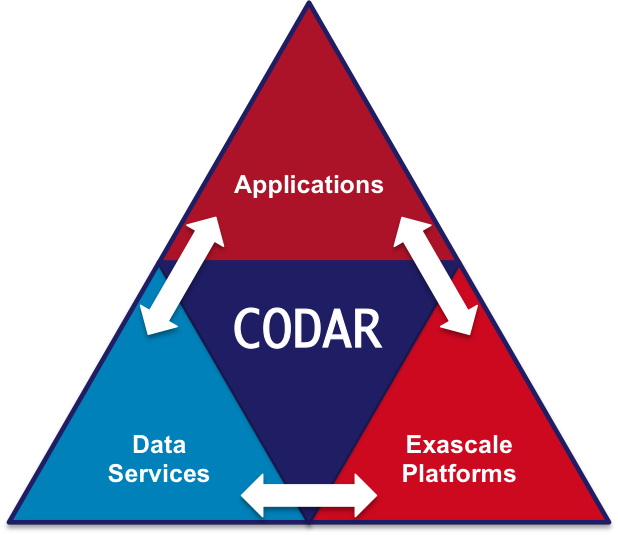
\includegraphics[width=3in]{Figs/CODAR.png}
\end{center}

\vspace{1in}




\newpage

\renewcommand{\contentsname}{{\huge Table of contents}}

\tableofcontents

\clearpage
\maketitle

\pagestyle{plain}
\setcounter{page}{1}

\section{Introduction}

Because of the vast volume of data being produced by today's scientific simulations and experiments, lossy data compressor allowing user-controlled loss of accuracy during the compression is a relevant solution for significantly reducing the data size. However, lossy compressor developers and users are missing a tool to explore the features of scientific data sets and understand the data alteration after compression in a systematic and reliable way. To address this gap, we will design and implement a generic framework called Z-checker, such that the users/developers can conveniently select the best-fit, adaptive compressors for different data sets. On the one hand, Z-checker combines a battery of data analysis components for data compression. On the other, Z-checker is implemented as an open-source community tool to which users and developers can contribute and add new analysis components based on their additional analysis demands. In this paper, we present a survey of existing lossy compressors. Then we describe the design framework of Z-checker, in which we integrated evaluation metrics proposed in prior work as well as other analysis tools. Specifically, for lossy compressor developers, Z-checker can be used to characterize critical properties such as entropy, distribution, power spectrum, principal component analysis, and autocorrelation) of any data set to improve compression strategies. For lossy compression users, Z-checker can detect the compression quality (compression ratio, bit rate), provide various global distortion analysis comparing the original data with the decompressed data (PSNR, normalized MSE, rate-distortion, rate-compression error, spectral, distribution, derivatives) and statistical analysis of the compression error (maximum, minimum, and average error, autocorrelation, distribution of errors). Z-checker is also a flexible framework, whose assessment library can be extended with more plugins coded in other programming languages or libraries, such as R and FFTW3. Z-checker provides two alternative execution modes: offline mode or online mode. The offline mode allows users to do the data compression assessment based on generated raw data files or existing decompressed data files. The online mode allows performing an in-situ analysis with running applications. Z-checker also features a visualization interface displaying all analysis results in addition to some basic views of the data sets such as time series.

\section{Stakeholders}

We list here potential stakeholders for this software and the results of any consultations that we have had with those stakeholders in developing this design document.

\subsection{Exascale applications}

ECP application (AD) projects demanding lossy compression techniques are a primary source of the codesign problems that Z-checker is designed to address.
We have consulted with many but certainly not all ECP AD teams to understand their requirement on data compression.

\subsection{Software technologies}

ECP software technology (ST) projects such as ADIOS, SZ, ZFP, Cinema, ALPINE, VTK-m, and Spack
are all potential contributors of software components that may be integrated into Z-checker assessment tool. 
Up to now (Jan. 2018), SZ and ZFP have been integrated into Z-checker. Z-checker has been integrated into ADIOS to a certain extent. 
For other projects/software components, we need to understand any constraints or special requirements that they may impose.
We intend to consult with many of those projects in developing this document.

\subsection{Hardware technologies}

Hardware technologies are a secondary primary source of the codesign problems that Cheetah is designed
to address. We have not as yet consulted with hardware projects.


\section{Use cases}

Use cases capture the user stories that motivate the work. As mentioned previously, Z-checker is a flexible 
framework that provides two execution modes based on users' diverse demands for compression assessment and
can be extended by adding compressors and analysis function libraries. 
We first introduce the use cases related to execution modes, then describe the use case of integrating lossy compressors into Z-checker, and finally summarize the ECP applications already assessed using Z-checker.

\subsection{Offline analysis}

Z-checker provides a series of executables for science users to perform the assessment based on the existing data files that were already produced by simulations. Specifically, given original raw data files, compressed data files, and decompressed data files, the user can perform the analysis by different commands, such as \emph{analyzeDataProperty}, \emph{compareDataSets}, \emph{runOfflineCase}, \emph{generateGNUPlot}, and \emph{generateReport}.
\begin{itemize}
  \item \emph{analyzeDataProperty} outputs the property information of the target data, such as value range, auto correlation, entropy values, and frequency information.
  \item \emph{compareDataSets} receives two input files (original raw file and decompressed file) and outputs the data distortion information between them (such as maximum error, distribution of errors, auto correlation of errors, and peak signal-to-noise ratio).
  \item \emph{runOfflineCase} integrates \emph{analyzeDataProperty} and \emph{compareDataSets}. It allows users to specify a set of data files and decompressed data files to the offline analysis in a batch way and provides multiple options allowing users to do the analysis with different levels/granularities.
  \item \emph{generateGNUPlot} allows to generate the evaluation figures (in .eps format) based on the analysis.
  \item \emph{generateReport} allows to generate the assessment report (in .pdf format) based on the analysis.
\end{itemize}

\subsection{Online analysis}

The SZ compressor provides a set of easy-to-use APIs for other developers (such as ADIOS developers) to integrate Z-checker's assessment functions. Online analysis is a typical use case allowing users to integrate Z-checker's API functions into their codes and run their applications/tools with Z-checker in parallel.

To activate the MPI version of Z-checker, the user needs to install an mpi library such as MPICH and adopt the ``--enable-mpi'' option during the installation of Z-checker. We provide examples for parallel data analysis and for parallel compression assessment. The user then needs to switch executionMode from OFFLINE to ONLINE in the configuration file (i.e., zc.config) or set the global variable ``executionMode'' to be ZC\_ONLINE during the initialization (SZ\_Init()).

The user needs only to specify the starting point and ending point of the compression and decompression by using Z-checker's interface in order to obtain the online assessment results. The related interfaces are listed below:
\begin{itemize}
  \item ZC\_DataProperty* dataProperty = ZC\_startCmpr(propName, ZC\_DOUBLE, g, 0, 0, 0, nbLines, M); //start compression
  \item ZC\_CompareData* compareResult = ZC\_endCmpr(dataProperty, cmprSize); //end compression
  \item ZC\_startDec(); //start decompression
  \item ZC\_endDec(compareResult, cmprCaseName, decData); //end decompression
\end{itemize}

An example is shown below:
\begin{lstlisting}[style=CStyle, basicstyle = \footnotesize\ttfamily]
for (i = 0; I < ITER_TIMES; i++) {
    localerror = doWork(nbProcs, rank, M, nbLines, g, h); //perform the simulation
    if(i%50==0) //control the compression frequency over time steps
    {
        //make a name for the current target data property
    	sprintf(propName, "%s_%04d", varName, i);
    	ZC_DataProperty* dataProperty = ZC_startCmpr(propName, ZC_DOUBLE, \
                    g, 0, 0, 0, nbLines, M); //start compression
    	cmprBytes = SZ_compress(SZ_DOUBLE, g, &cmprSize, 0, 0, 0, nbLines, M);
        //end compression
    	ZC_CompareData* compareResult = ZC_endCmpr(dataProperty, cmprCaseName, cmprSize);
    	sprintf(cmprCaseName, "%s_%s_%04d(1E-3)", varName, compressorName, i);
    	ZC_startDec(); //start decompression
    	decData = SZ_decompress(SZ_DOUBLE,cmprBytes,cmprSize,0,0,0,nbLines,M);	
    	ZC_endDec(compareResult, decData); //end decompression			

    	if(rank==0)
    		ZC_writeDataProperty(dataProperty, "dataProperties");
    	
        //free data property generated at current time step		
    	freeDataProperty(dataProperty);
        //free compression assessment results at current time step
    	freeCompareResult(compareResult);
    	free(cmprBytes);
    	free(decData);
    }
    //Aggregate the residual for checking if the loop meets the convergence condition
    if ((i%REDUCE) == 0) {
    	MPI_Allreduce(&localerror,&globalerror,1,MPI_DOUBLE,MPI_MAX,MPI_COMM_WORLD);
    }
    if(globalerror < PRECISION) {
    	break;
    }
}

\end{lstlisting}

\subsection{ECP applications assessed by Z-checker}

\begin{itemize}
  \item ExaSky (HACC cosmology simulation and NYX cosmology simulation)
  \item QMCPack (quantum chemistry simulation)
  \item EXAALT (molecular dynamics simulation)
  \item EXAFEL (Linac Coherent Light Source)
  \item NWCHEM-X (NWCHEM data sets)
  \item GAMESS (two-integrals data sets)
\end{itemize}


\section{Requirements}

\emph{We extract requirements from stakeholder interviews and use cases.}

\begin{enumerate}[label=R-\arabic*)]
\item
Z-checker should be able to run experiments on MIRA, Titan, Theta, and more systems.
\item
Z-checker should be able to run experiments on both Linux workstations and MacOS.
\item
Z-checker should be able to run the application with alternative reduction algorithms with tunable parameter settings.
\item
Z-checker should be able to collect and output data distortion results.
\item 
Z-checker should be able to collect and output reduction performance results.
\item 
Z-checker should be able to support different I/O libraries/formats, such as HDF5, NetCDF, Adios.
\item
Z-checker should be able to provide two execution modes, online and offline. 
\item
Z-checker should be able to support integration with more math libraries such as R and FFTW3. 
\end{enumerate}


\section{Related work}

\emph{Here we describe related studies.}

Baker et al. \cite{baker} investigated the use of data compression techniques on climate simulation data from CESM \cite{cesm}. They developed an approach for verifying the climate data and used it to evaluate several compression algorithms, including FPZIP \cite{fpzip}, ISABELA, APAX, and GRIB2 (with JPEG2000 compression). The verification process included (1) quantifying the difference between the original and reconstructed data sets via measures of pointwise error, average error (RMSE and NRMSE), and Pearson correlation and (2) evaluating the reconstructed data in the context of an ensemble of CESM runs with slight perturbations by a CESM port verification tool (CESM-PVT). They determined that the diversity of the climate data requires individual treatment of variables and that the reconstructed data can fall within the natural variability of the system.
Laney et al. \cite{laney2014assessing} examined the effects of lossy compression in physics simulations by evaluating two lossy compressors (FPZIP and APAX \cite{apax}) in three physics simulation codes. They used physics-based metrics for each simulation to assess the impact of lossy compression. They noted that the characteristics of the compression error must be carefully considered in the context of the underlying physics being modeled.
Lakshminarasimhan et  al. \cite{isabela} propose the ISABELA lossy compressor. It performs data compression by B-spline interpolation after sorting the data series. They evaluated the performance of ISABELA with several metrics: compression ratio, maximum compression error (pointwise relative error), average compression error (NRMSE), and compression time. They also evaluated the compressed data by quantitative analysis and visual analysis. In quantitative analysis, they evaluated the Pearson correlation of different data regions and the difference of derived data. In visual analysis, they utilized the visualization tool to present the original data and ISABELA-compressed data.
Lindstrom \cite{zfp} proposed a lossy compression algorithm for floating-point arrays in fixed rate (i.e. ZFP) and evaluated ZFP of rate-distortion, rate speed, density spectrum, and derivatives (Morse segmentation of gradients) in several applications, including quantitative and visual analysis, visualization, and fluid dynamics simulation.
Sasaki et al. \cite{ssem} proposed a lossy compression method (i.e. SSEM) based on wavelet transform and vector quantization. They applied their compression method to a checkpoint/restart technique and evaluate the impact on results of a production climate application (NICAM).
Di and Cappello \cite {sz} proposed an error-bounded lossy compressor (i.e. SZ) based on curve-fitting and binary representation analysis. They evaluated SZ with the metrics including the maximum compression error (bounded or not bounded), compression ratio, and compression/decompression speed.


\section{Design}

We introduce the design framework and some implementation details.

\subsection{Overview}
Z-checker is a novel framework with three important features: (1) it can be used to explore the properties of original data sets for the purpose of data analytics or improvement of lossy compression algorithms; (2) it is integrated with a rich set of evaluation algorithms and assessment functions for selecting best-fit lossy compressors for specific data sets; and (3) it features both static data visualization scripts and an interactive visualization system, which can generate visual results on demand. This interactive mode allows compression algorithm developers and users to dynamically compute analyses on user-selected portions of the data set.

Z-checker is designed to support two processing modes, on-line and off-line, and two display modes, static and interactive. The four modes correspond to four different use cases. The off-line static mode is useful for generating a report on the original data set properties and the compression error, presenting multiple analysis views. The off-line interactive mode is useful for exploring the properties of the original data sets and the compression error. It allows users to dig into some region of interest and reveal local properties that are not present or visible on the whole data set. The on-line static display mode corresponds to in situ data compression and may generate and update the original data set compression analysis as long as the data is presented to Z-checker. The on-line interactive mode allows users to monitor the compression error while the data is produced. Users can zoom in on regions of interest and assess the quality of the data compression. Table \ref{tab:modes} summarizes the four use cases of Z-checker, considering the two processing modes and two visualization modes.

\begin{table}[ht] \centering
\caption{Four Use Cases of Z-checker} \centering
\scriptsize
\begin{tabular}{|l|p{0.315\columnwidth}|p{0.315\columnwidth}|}
\hline \multicolumn{1}{|c|}{} & \multicolumn{1}{|c|}{Off-line Processing}&\multicolumn{1}{|c|}{On-line Processing}\\
\hline
Static Display & Load data once and view results by generating local image files. & Load data based on dynamic requests and view results by  local image files.\\
\hline
Interactive Display & Load data once and view results on demand via a web page interactively. & Load data dynamically and view results on demand by a web page interactively. \\
\hline
\end{tabular}
\label{tab:modes}
\end{table}

 \begin{figure}[ht] \centering
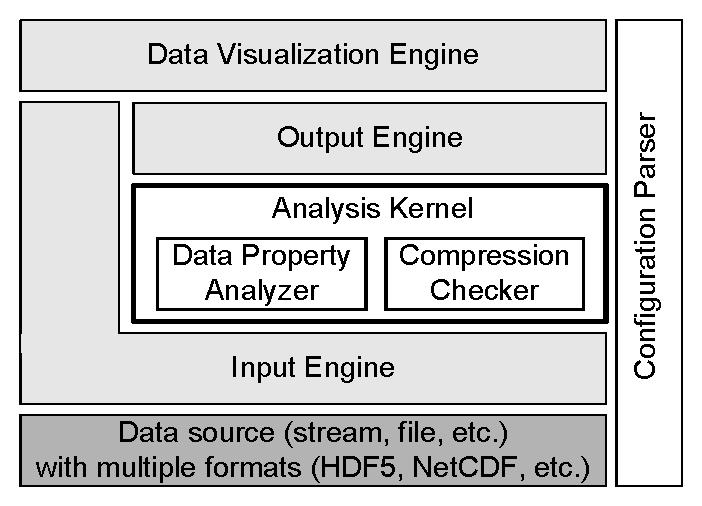
\includegraphics[scale=.6]{Figs/framework.eps}
\caption{Design Architecture of Z-checker}
\label{fig:framework}
\end{figure}

The design architecture of Z-checker is presented in Figure \ref{fig:framework}, which involves three critical parts: \emph{user interface},  \emph{processing module}, and \emph{data module}.
\begin{itemize}
\item \emph{User interface} includes three key engines---input engine, output engine, and data visualization engine---as shown in the light-gray rectangles in Figure \ref{fig:framework}. They are in charge of reading the floating-point data stream (either original data or compressed bytes), dumping the analyzed data to disks/PFS, and plotting data figures for visualizing analysis results. The Data visualization engine also provides the interactive mode through a web browser interface (details are described later).
\item \emph{Processing module} is the core module in the framework, which includes the analysis kernel and configuration parser. The former is responsible for performing the critical analysis, and the latter is in charge of parsing the user's analysis requirements (such as specifying the input file path, the compression command or executable, and the customization for the analysis metrics on demand). Specifically, the analysis kernel is composed of two critical submodules, the data property analyzer and compression checker, which are responsible for exploring data properties based on the original data sets and analyzing the compression results with specified lossy compressors (discussed later in more detail).
\item \emph{Data source module}, the dark-gray box in the figure, is the bottom layer in the framework and represents the data source (such as the data stream produced by scientific applications at runtime or the data files stored in the disks).
\end{itemize}

\subsection{Terminology}

\begin{description}

\item[Application:] An executable program with a specific science purpose and a
designated input and output format. A given application may have multiple
executables for different target architectures and for testing different
compiler optimizations, but each such executable must have consistent
parameter, input, and output formats.

\item[Application run:] A run of an application with a given set of parameters

\item[Lossy compressor:] The library that provides the lossy compression capability for scientific data sets. The science data includes different types, such as integer, single-precision and double-precision floating-point data. A lossy compressor should provide both executables and APIs for different users to call the lossy compression functions. A good lossy compressor should also provide multiple options for users to control compression errors and it should respect the compression errors based on the specified error control.

\item[Compression quality:] Compression quality includes compression ratio, bit-rate, compression time, decompression time, data distortion, rate-distortion, and so on. Compression ratio is defined as the ratio of the original raw data size to the the size of the compressed data. Bit-rate refers to the number of bits used to represent one data point after the compression. Hence, bit-rate is equal to the ratio of the number of bits used by one data point originally (e.g., 64 for double-precision floating-point data) to the compression ratio. Compression and decompression time are usually evaluated by compression rate and decompression rate respectively. Compression rate is the ratio of the original raw data size (in MB) to the compression time (in seconds). The decompression rate is the ratio of the original raw data size (in MB) to the decompression time (in seconds). Data distortion involves a set of distortion metrics such as maximum compression errors and peak signal-to-noise ratio (PSNR). Rate distortion is a common metric to evaluate the compression quality. Rate, here, means the bit-rate; distortion refers to PSNR.


\item[Offline analysis:] Offline analysis means that given specific raw data files, compressed data files, and/or decompressed data files, Z-checker is able to perform the analysis and generate a report.

\item[Online analysis:] Online analysis means that Z-checker will be integrated into other tools or applications, performing the analysis while the application is running and generating the assessment report in the end.

\end{description}

\subsection{Dependencies}

Some functionality in Z-checker depends on third-party libraries, which are listed as follows:

\begin{enumerate}
\item Support MPI library: ./configure --prefix=[install\_dir] --enable-mpi . (The user needs to install MPI library such as MPICH in advance.)
\item Support NetCDF : usage can be found in the subdirectory NetCDFReader/ (./configure --prefix=[install\_dir] --enable-netcdf --with-netcdf-prefix=DIR; NetCDF needs to be installed in advance.)
\item Support HDF5 library: details can be found in HDF5Reader/ (./configure --prefix=[install\_dir] --enable-hdf5; the user needs to install HDF5 and set its environment variables according to the HDF5 guide in advance.)
\item Support FFTW3 library: computation of 3D auto correlation requires FFTW3. In particular, 3D auto correlation is computed by using some functions provided by FFTW3. (./configure --prefix=[indall\_dir] --enable-fftw3 --with-fftw3-prefix=DIR; the user ndeeds to install FFTW3 in advance.)
\item Support R language/library: the functions coded in R scripts can be executed in the data analysis and compression analysis. In particular, the SSIM function is coded in R and requires the R library in Z-checker. (./configure --prefix=[index\_dir] --enable-r --with-r-prefix=DIR)
\end{enumerate}

In addition, the user can also use --with-xxx-include-path and --with-xxx-lib-path to specify the header directory and lib directory, respectively, instead of --with-xxx-prefix. More options can be found by executing "./configure -help".

\subsection{Z-checker command line format and basic usage}

\textbf{Command}: runOfflineCase\\
Description: This is a command to execute the offline analysis based on given data files and compressed/decompressed data files.
\begin{lstlisting}[style=ShellStyleInline, basicstyle = \footnotesize\ttfamily]
Usage: runOfflineCase <options>
Options:
* input information:
    -N <compressor name>: the name of the compressor
    -C <information file> : the file containing the data information
* analysis options:
    -A : perform the full analysis of the compression results
    -a <metric> : perform quick analysis for specific metric
        *metric options: (including all variables)
          cr  : compression ratio (min, avg, max)
          err : compression error (min, avg, max)
          full: complete information listed as above
* metadata options:
    -n : print number of variables
    -m : print the names of variables
    -l : list complete information of all variables
    -p : print all the precisions used in the analysis
* Examples:
    runOfflineCase -C varCmpr.inf -l
    runOfflineCase -C varCmpr.inf -m
    runOfflineCase -C varCmpr.inf -A
    runOfflineCase -C varCmpr.inf -a err
    runOfflineCase -C varCmpr.inf -a cr
\end{lstlisting}

\textbf{Command}: zccallr\\
Description: This executable is for users to simply test the execution of R script files. zccallr.c is a good example to show how to call an R script from C.
\begin{lstlisting}[style=ShellStyleInline, basicstyle = \footnotesize\ttfamily]
Usage: zccallr <options>
Options:
* Rscript file:
	-s <script_file>: specify the path of the R_script_file
	-c <function_name>: specify the function
* data type:
	-i : integer data (int type)
	-f : single precision (float type)
	-d : double precision (double type)
* input data files:
	-e <endian_type>: endian type of the binary data in input files:
				0(little-endian); 1(big-endian)
	-A <first data file> : first data file such as original data file
	-B <second data file> : second data file such as decompressed data file
	-C <third data file> : third data file for analysis
	-D <fourth data file> : fourth data file for analysis
	-E <fifth data file> : fifth data file for analysis
	-F <sixth data file> : sixth data file for analysis
* output type of result file:
	-r : print the result on the screen.
	-b : analysis result stored in binary format
	-t : analysis result stored in text format
	-o <output file path> : the path of the output file.
* dimensions:
	-1 <nx> : dimension for 1D data such as data[nx]
	-2 <nx> <ny> : dimensions for 2D data such as data[ny][nx]
	-3 <nx> <ny> <nz> : dimensions for 3D data such as data[nz][ny][nx]
* examples:
	zccallr -s func.R -c add1 -r -f -e 0 \
		-A ../../examples/testdata/x86/testfloat_8_8_128.dat \
				-3 8 8 128
	zccallr -s func.R -c computeErr -r -f -e 0 \
		-A ../../examples/testdata/x86/testfloat_8_8_128.dat \
		-B ../../examples/testdata/x86/testfloat_8_8_128.dat.sz.out \
		-3 8 8 128
\end{lstlisting}

\subsection{Z-checker configuration files}

1. zc.config (specifying the metrics to be used in the assessment)

This configuration file is used by many commands in Z-checker, such as analyzeDataProperty and compareDataSets.
\begin{lstlisting}[style=ShellStyleInline, basicstyle =\footnotesize\ttfamily]
#============================================================
[ENV]
#the path of the R script for special analysis such as KS_test and SSIM
#automatically set during the running of examples/Makefile
RscriptPath = /home/sdi/Z-checker/R/test/data_analysis_script.R

#endianType: either LITTLE_ENDIAN_DATA or BIG_ENDIAN_DATA
#x86, x64 and arm adopt LITTLE_ENDIAN_DATA
#PowerPC (PPC), MAC OS, and KEIL C51 adopt BIG_ENDIAN_DATA
dataEndianType = LITTLE_ENDIAN_DATA

#two statuses: either PROBE (used in detecting/monitoring compression
#results during compression) or ANALYZER (used in gleaning the results
#for plotting and analysis)
#example: checkingStatus = PROBE_COMPRESSOR
#example: checkingStatus = ANALYZE_DATA
#example: chekcingStatus = COMPARE_COMPRESSOR
checkingStatus = PROBE_COMPRESSOR

#two options for execution mode: either ONLINE or OFFLINE;
#ONLINE means running with parallel application such as MPI programs to
#check the compression at runtime (the data are produced by simulations at runtime)
#OFFLINE means running separately from the user application (the data are loaded
#from the files which are already in the disks)
executionMode = ONLINE

[DATA]
#to analyze the properties of the single data set

#compute minimal value of the data set? (1:yes, 0:no)
minValue = 1
#compute maximal value of the data set?
maxValue = 1
#value range of the data set?
valueRange = 1
#average value of the data?
avgValue = 1
#compute entrpy?
entropy = 1
#compute auto correlation of the data (to check smoothness)?
autocorr = 1
#compute 3D auto correlation of the data (to check smoothness)
autocorr3D = 1
#generate coefficients of the FFT transform?
fft = 1
#generate analysis for laplace
lap = 0

[COMPARE]
#To compare two data sets (e.g., original data vs. decompressed data)

#compression time & compression rate
compressTime = 1
#decompression time & decompression rate
decompressTime = 1
#compression size
compressSize = 1

#compute minimal absolute error between the two data sets
minAbsErr = 1
#compute average absolute error between the two data sets
avgAbsErr = 1
#compute maximal absolute error between the two data sets
maxAbsErr = 1
#compute the auto correlation of the absolute errors (white noises?)
autoCorrAbsErr = 0
#compute the 3D auto correlation of the absolute errors
autoCorrAbsErr3D = 0
#compute the PDF of the absolute errors
absErrPDF = 1
#compute the PDF of the pwr errors
pwrErrPDF = 0

#compute the value-range based minimal relative error
minRelErr = 1
#compute the value-range based average relative error
avgRelErr = 1
#compute the value-range based maximal relative error
maxRelErr = 1

#compute root mean squared error
rmse = 1
#compute normalized root mean squared error (NRMSE)
nrmse = 1
#compute peak signal-to-noise ratio (PSNR)
psnr = 1
#compute signal-to-noise ratio (SNR)
snr = 1

#compute the pearson correlation between the original data values and the
#compression errors
valErrCorr = 1

#compute the pearson correlation coefficient between the two data sets
#(to check five "nine"s?)
pearsonCorr = 1

[PLOT]
#plot the figures based on the data across different compressors or variables

#extension of property_files, which are under compressors_dir/dataProperties
propertyExtension = prop

plotAutoCorr = 1
plotFFTAmp = 1
plotEntropy = 1

plotCompressionResults = 1

plotAbsErrPDF = 1
\end{lstlisting}

2. varCmpr.info (specifying the data files to be involved in the assessment)

This configuration file is used by runOfflineCase command.
As follows, we present an example configuration file to specify a set of existing data files for assessment.
\begin{itemize}
  \item ori\_data: original data file
  \item prec: precision of the compression (such as error bound)
  \item cpr\_time: compression time (manually set by users)
  \item dec\_time: decompression time (manually set by users)
  \item cpr\_data: the path of the compressed data file
  \item dec\_data: the path of the decompressed data file
\end{itemize}
\begin{lstlisting}[style=ShellStyleInline, basicstyle =\footnotesize\ttfamily]
#information about the variables and compression demands
ori_data=CLDHGH_1_1800_3600:LITTLE_ENDIAN:FLOAT:1800x3600:../runOfflineCase_testdata/CLDHGH_1_1800_3600.dat
prec=1E-3
cpr_time=0.2
dec_time=0.1
cpr_data=../runOfflineCase_testdata/CLDHGH_1_1800_3600_1E-3.dat.sz
dec_data=../runOfflineCase_testdata/CLDHGH_1_1800_3600_1E-3.dat.sz.out
prec=1E-4
cpr_time=0.4
dec_time=0.2
cpr_data=../runOfflineCase_testdata/CLDHGH_1_1800_3600_1E-4.dat.sz
dec_data=../runOfflineCase_testdata/CLDHGH_1_1800_3600_1E-4.dat.sz.out
prec=1E-5
cpr_time=0.8
dec_time=0.4
cpr_data=../runOfflineCase_testdata/CLDHGH_1_1800_3600_1E-5.dat.sz
dec_data=../runOfflineCase_testdata/CLDHGH_1_1800_3600_1E-5.dat.sz.out
prec=1E-6
cpr_time=1.2
dec_time=0.6
cpr_data=../runOfflineCase_testdata/CLDHGH_1_1800_3600_1E-6.dat.sz
dec_data=../runOfflineCase_testdata/CLDHGH_1_1800_3600_1E-6.dat.sz.out

ori_data=CLDLOW_1_1800_3600:LITTLE_ENDIAN:FLOAT:1800x3600:../runOfflineCase_testdata/CLDLOW_1_1800_3600.dat
prec=1E-3
cpr_time=0.2
dec_time=0.1
cpr_data=../runOfflineCase_testdata/CLDLOW_1_1800_3600_1E-3.dat.sz
dec_data=../runOfflineCase_testdata/CLDLOW_1_1800_3600_1E-3.dat.sz.out
prec=1E-4
cpr_time=0.4
dec_time=0.2
cpr_data=../runOfflineCase_testdata/CLDLOW_1_1800_3600_1E-4.dat.sz
dec_data=../runOfflineCase_testdata/CLDLOW_1_1800_3600_1E-4.dat.sz.out
prec=1E-5
cpr_time=0.8
dec_time=0.4
cpr_data=../runOfflineCase_testdata/CLDLOW_1_1800_3600_1E-5.dat.sz
dec_data=../runOfflineCase_testdata/CLDLOW_1_1800_3600_1E-5.dat.sz.out
prec=1E-6
cpr_time=1.2
dec_time=0.6
cpr_data=../runOfflineCase_testdata/CLDLOW_1_1800_3600_1E-6.dat.sz
dec_data=../runOfflineCase_testdata/CLDLOW_1_1800_3600_1E-6.dat.sz.out
\end{lstlisting}

3. errBounds.cfg (specifying the error bounds used in the assessment)

This configuration is used by only One-command assessment of Z-checker-installer.
\begin{lstlisting}[style=ShellStyleInline, basicstyle =\footnotesize\ttfamily]
#Compression error bounds for SZ
SZ_ERR_BOUNDS="1E-1 1E-2 1E-3 1E-4"

#Compression error bounds for ZFP
ZFP_ERR_BOUNDS="1E-1 1E-2 1E-3 1E-4"

#Compression cases used to compare two compressors
comparisonCases="sz_f(1E-2),sz_d(1E-2),zfp(1E-2) sz_f(1E-4),sz_d(1E-4),zfp(1E-4) sz_f(1E-6),sz_d(1E-6),zfp(1E-6)"

#Number of evaluation results to be shown in the report
numOfErrorBoundCases="2"
\end{lstlisting}

\subsection{output directory layout}

\begin{lstlisting}[style=ShellStyleInline, basicstyle =\footnotesize\ttfamily]

dataProperties
    variable_1.prop         #basic property analysis results of variable 1
    variable_1.autocorr     #auto correlation of variable 1
    variable_1.lap          #lapalace results of variable 1
    variable_1.fft          #FFT transform coefficients (real and imag)
    variable_1.fft.amp      #amplitude of FFT transform
    variable_1.autocorr3d   #3D auto correlation of variable 1
    .....
    variable_N.prop         #basic property analysis results of variable N
    variable_N.autocorr     #auto correlation of variable N
    variable_N.lap          #lapalace results of variable N
    variable_N.fft          #FFT transform coefficients (real and imag)
    variable_N.fft.amp      #amplitude of FFT transform
    variable_N.autocorr3d   #3D auto correlation of variable N

compressionResults
    compressor:variable.cmp         #basic compression results
    compressor:variable.dis         #distribution of compression errors
    compressor:variable.fft         #FFT transform results of decompressed data
    compressor:variable.fft.amp     #FFT transform amplitudes of decompressed data
    compressor:variable.autocorr    #auto correlation of compression errors
    compressor:variable.autocorr3d  #3D auto correlation of compression errors
\end{lstlisting}

\subsection{One-command installation and usage}

We provide a very easy-to-use way for users to install and use Z-checker, by leveraging Z-checker-installer. In Z-checker-installer, one user can perform only one command (i.e., z-checker-install.sh) to install every related depending package or libraries, such as SZ, ZFP, gnuplot, latex. After the simple installation, the user just needs to execute two commands to finish the complete assessment procedure for a given data set. (1) Executing \emph{createZCCase.sh} can generate an individual workspace based on the user's specified test case name. (2) Executing \emph{runZCCase.sh} will perform the compression automatically by different compressors such as SZ and ZFP, and finally generate the assessment report with narratives and figures insides.
in the future, If the user wants to update his/her package based on the already installed z-checker-installer, he/she can execute one command z-checker-update.sh for simplicity, instead of rerunning z-checker-install.sh.

Both Z-checker tool and Z-checker-installer package will be put in Spack later.

\subsection{A typical test plan}

This example describes how to generate data property analysis results and compression results, given original data files (in binary), compressed files and decompressed files.

\begin{lstlisting}[style=ShellStyleInline, basicstyle =\footnotesize\ttfamily]

#Use createOfflineCase.sh to create a use-case directory, which will contain
#all the executables. Then, do the following steps.
#Preparing the testing data
.1. Download the testing data from here:
http://www.mcs.anl.gov/~shdi/download/runOfflineCase_testdata.tar.gz
#Tips: the testing data package contains two original data files and their
#corresponding SZ-compressed files and decompressed files based on different
#error bounds
.2. tar -xzvf runOfflineCase_testdata.tar.gz

#Generate the property analysis results and compression results
.3. ./createOfflineCase.sh testcase1
.4. cd testcase1
.5. ./runOfflineCase -C varCmpr.inf -A -N sz
#Tips: More options can be shown by executing ./runOfflineCase without any input
#options; in the above example, we set the compress name as "sz" because the
#compressed/decompressed data files were generated by sz.

#Generate figures based on the property/compression results in form of GNUPlot
.6. Edit zc.config as follows:
    compressors = sz:[the absolute path of the directory of the test case]
#Tips: sz here refers to the compressor name. You can replace it by your
#own compressor
    comparisonCases = sz(1E-3)
.7. ./generateGNUPlot zc.config
#Then, you can find rate-distortion eps files generated in the current directory.
#More information can be found in the doc/userguide.pdf
#Tips: You can run the executables or scripts without any inputs to see
#the help information
\end{lstlisting}

\subsection{Release Goals}
Release 0.2 for June 2018 will consist of the following functionalities.

\begin{itemize}
  \item Support both online and offline analysis
  \item Support reading of HDF5, NetCDF, Adios data
  \item One-command installation and assessment
  \item Support integration of 3rd-party libraries
  \item Z-checker web visualization
  \item Evaluation reports generated by Z-checker
\end{itemize}

\section{Metrics}

The purpose of Z-checker is to perform all the compression-related assessment on real science applications
to allow the developers to select either the best-fit compressors for specific applications or improve the compression quality, particularly on 
exascale architectures. The metrics will be the number of applications assessable by Z-checker, the number of I/O libraries Z-checker supports, our understanding of the compression quality based on Z-checker, and our success at improving compressors.


\section{Work plan}

\begin{tabular}{|p{0.7in}|p{5.5in}|}\hline
\textbf{Date}  & \textbf{Milestone} \\\hline
3/31/2017 & Final design document for Z-checker v0.1 \\\hline
6/30/2017 & Z-checker v0.1.0 (support offline analysis)\\\hline
12/15/2017 & Z-checker v0.1.1 (support offline analysis)\\\hline
1/31/2018 & Final design document for Z-checker v0.2 \\\hline
1/31/2018 & Z-checker v0.1.2 (support online analysis partially)\\\hline
6/30/2018 & Z-checker v0.1.3 (support full online analysis) \\\hline
12/14/2018 & Z-checker v0.2 \\\hline
\end{tabular}

\section{Open questions}

\begin{itemize}
\item
How do various compressors set parameters?

\item
How to implement parallel version for some complicated assessment algorithms, such as FFT and auto-correlation of errors?

\item 
How to implement parallel algorithms (online analysis) based on external calls of third-party libraries such as R language? 
\end{itemize}



\clearpage
\bibliographystyle{ieeetr}
\bibliography{Bibs/z-checker.bib}

\end{document}

